% AgenticScientist: method report for the Virtual Embryo Challenge 2026 (Agent track).
% Compile with pdfLaTeX. Figures: fig/*.pdf (made by figs.py from data/*.json) and fig_architecture.tex (TikZ).
\documentclass[9pt,twocolumn,a4paper]{extarticle}
\usepackage[T1]{fontenc}
\usepackage[utf8]{inputenc}
\usepackage{textcomp}
\usepackage{newtxtext,newtxmath}
\usepackage[scaled=0.9]{helvet}
\usepackage[a4paper,textwidth=180mm,textheight=247mm,columnsep=6.5mm,headsep=5mm,footskip=8mm]{geometry}
\usepackage{microtype}
\usepackage{graphicx}
\usepackage{xcolor}
\usepackage{booktabs,tabularx,array,multirow}
\usepackage{amsmath}
\usepackage{enumitem}
\usepackage{titlesec}
\usepackage{fancyhdr}
\usepackage[font={sf,footnotesize},labelfont={bf},labelsep=space,justification=justified,singlelinecheck=false,skip=5pt]{caption}
\usepackage{stfloats}
\usepackage{tikz}
\usetikzlibrary{arrows.meta,positioning,calc,fit,backgrounds}
\usepackage[colorlinks=true,linkcolor=asblue!80!black,citecolor=asblue!80!black,urlcolor=asblue!80!black]{hyperref}
\definecolor{asblue}{HTML}{2A78D6}
\definecolor{asorange}{HTML}{EB6834}
\definecolor{asaqua}{HTML}{1BAF7A}
\definecolor{asyellow}{HTML}{EDA100}
\definecolor{asink}{HTML}{0B0B0B}
\definecolor{asinktwo}{HTML}{52514E}
\definecolor{asmuted}{HTML}{898781}
\definecolor{aslane}{HTML}{F4F4F1}
\definecolor{asrule}{HTML}{C3C2B7}


% ---- layout details
\renewcommand{\figurename}{Fig.}
\captionsetup[figure]{name={Fig.}}
\captionsetup[table]{name={Table}}
\titleformat{\section}{\sffamily\bfseries\fontsize{10.5}{12.5}\selectfont\color{asink}}{\thesection}{0.6em}{}
\titleformat{\subsection}{\sffamily\bfseries\fontsize{9}{11}\selectfont\color{asink}}{\thesubsection}{0.6em}{}
\titleformat{\paragraph}[runin]{\sffamily\bfseries\fontsize{8.6}{10.5}\selectfont\color{asink}}{}{0em}{}[.]
\titlespacing*{\section}{0pt}{9pt plus 2pt minus 1pt}{3.5pt}
\titlespacing*{\subsection}{0pt}{7pt plus 2pt minus 1pt}{2.5pt}
\titlespacing*{\paragraph}{0pt}{4pt plus 1pt}{0.5em}
\setlength{\parindent}{1em}
\setlength{\parskip}{0pt}
\setlist{nosep,leftmargin=1.25em}
\pagestyle{fancy}
\fancyhf{}
\renewcommand{\headrulewidth}{0.4pt}
\renewcommand{\headrule}{\hbox to\headwidth{\color{asrule}\leaders\hrule height \headrulewidth\hfill}}
\fancyhead[L]{\sffamily\fontsize{7}{8}\selectfont\color{asinktwo}AgenticScientist \textbar{} Method report}
\fancyhead[R]{\sffamily\fontsize{7}{8}\selectfont\color{asinktwo}Virtual Embryo Challenge 2026 \textbar{} Agent track}
\fancyfoot[C]{\sffamily\fontsize{7.5}{8}\selectfont\color{asinktwo}\thepage}
\setlength{\headheight}{11pt}
\newcommand{\dev}{\textsc{Dev}}
\newcommand{\code}[1]{\texttt{\small #1}}
\newcommand{\tightcell}[1]{\begin{tabular}[t]{@{}l@{}}#1\end{tabular}}
\newcolumntype{L}[1]{>{\raggedright\arraybackslash}p{#1}}
\newcolumntype{Y}{>{\raggedright\arraybackslash}X}
\renewcommand{\arraystretch}{1.12}
\setlength{\textfloatsep}{11pt plus 2pt minus 2pt}
\setlength{\dbltextfloatsep}{11pt plus 2pt minus 2pt}
\setlength{\floatsep}{9pt plus 2pt minus 2pt}

\begin{document}

\twocolumn[{%
\begin{flushleft}
{\sffamily\fontsize{7.5}{9}\selectfont\color{asblue}\textbf{METHOD REPORT}\quad\color{asinktwo}Virtual Embryo Challenge, NeurIPS 2026 \textbullet{} Agent track \textbullet{} 26 November 2026\par}
\vspace{7pt}
{\sffamily\bfseries\fontsize{18.5}{22}\selectfont\color{asink}
AgenticScientist: a locked multi-model research harness with paired statistical acceptance and holdout-calibrated selection for forecasting mouse embryo development\par}
\vspace{8pt}
{\sffamily\fontsize{10}{12}\selectfont\color{asink}The AgenticScientist Team\par}
\vspace{2pt}
{\sffamily\fontsize{7.8}{9.5}\selectfont\color{asinktwo}Leaderboard entry: \emph{AgenticScientist Lab} (Agent track). Correspondence: via the challenge organisers.\par}
\vspace{9pt}
\noindent\colorbox{aslane}{\parbox{\dimexpr\textwidth-2\fboxsep\relax}{%
\vspace{3pt}\hspace*{4pt}\parbox{\dimexpr\textwidth-2\fboxsep-8pt\relax}{\sffamily\fontsize{8.6}{11.4}\selectfont\color{asink}
\textbf{Abstract.}
Autonomous research agents generate and implement far more hypotheses than a development leaderboard can safely
adjudicate. AgenticScientist, the harness behind our Agent-track entry to the Virtual Embryo Challenge, fixes every
input of a run in a cryptographic lock and lets sandboxed board workers iterate without human steering. A frontier
language model, rotated across vendors, writes one falsifiable hypothesis and implements it; a paired, seed-matched
race against the parent program decides acceptance; a second model audits the diff. Final programs are not chosen on
development scores. After research ends, shortlisted programs are re-scored on protected stages that no agent could
read, and a board's change is promoted only if its paired lower confidence bound beats the seed. Across four locked
runs, 41 development winners were re-scored in this way and 5 improved the holdout; on two of three boards
development gain and holdout gain were negatively correlated ($r=-0.89$ and $-0.83$). In the final run a
development-greedy composition would have gained 15.7 development points and lost 10.1 holdout points. The selected
composition gained 5.1 on both and scored 213.4 on the hidden test (rank 24 of 97 agent teams when submissions
closed). We also report a run that returned its seed unchanged, the predecessor runs that shaped the rules, and which
parts of the result are owed to the agents and which to the people who prepared the locks.
}\vspace{3pt}}}
\end{flushleft}
\vspace{6pt}
}]

% =====================================================================================================================
\section{Introduction}

Large language models can now run the whole inner loop of empirical research: read a brief, inspect data, propose a mechanism, implement it and interpret a score \cite{lu2024aiscientist,romera2024funsearch,novikov2025alphaevolve}. The bottleneck moves from generating ideas to deciding which of them are real. An agent that evaluates itself a hundred times a day on a fixed development set will find changes that raise the development score for reasons that do not hold on new data. This is the adaptive data analysis problem \cite{dwork2015reusable,blum2015ladder} at machine speed.

The Virtual Embryo Challenge \cite{vec2026} makes the problem concrete. Teams forecast held-out developmental stages
of the mouse embryo from earlier ones, the decisive targets lie two to three days beyond the last released stage, and
the Agent track forbids a person from steering the agent once a run has started. Whatever protects a run against
self-deception must be built into the harness before it is locked. AgenticScientist does this with four procedural
elements: a \textbf{run lock} that hashes every input and is re-verified every cycle; a \textbf{research cycle} in
which one sandboxed model designs and implements a single hypothesis; \textbf{paired racing acceptance} against the
parent program; and \textbf{holdout-calibrated selection}, which composes the final program board by board from
changes that beat the seed on protected stages. The last element mattered most.

% =====================================================================================================================
\begin{figure*}[t]
\centering
\resizebox{\textwidth}{!}{% Architecture of the AgenticScientist harness (TikZ). Included by main.tex; colours are defined there.
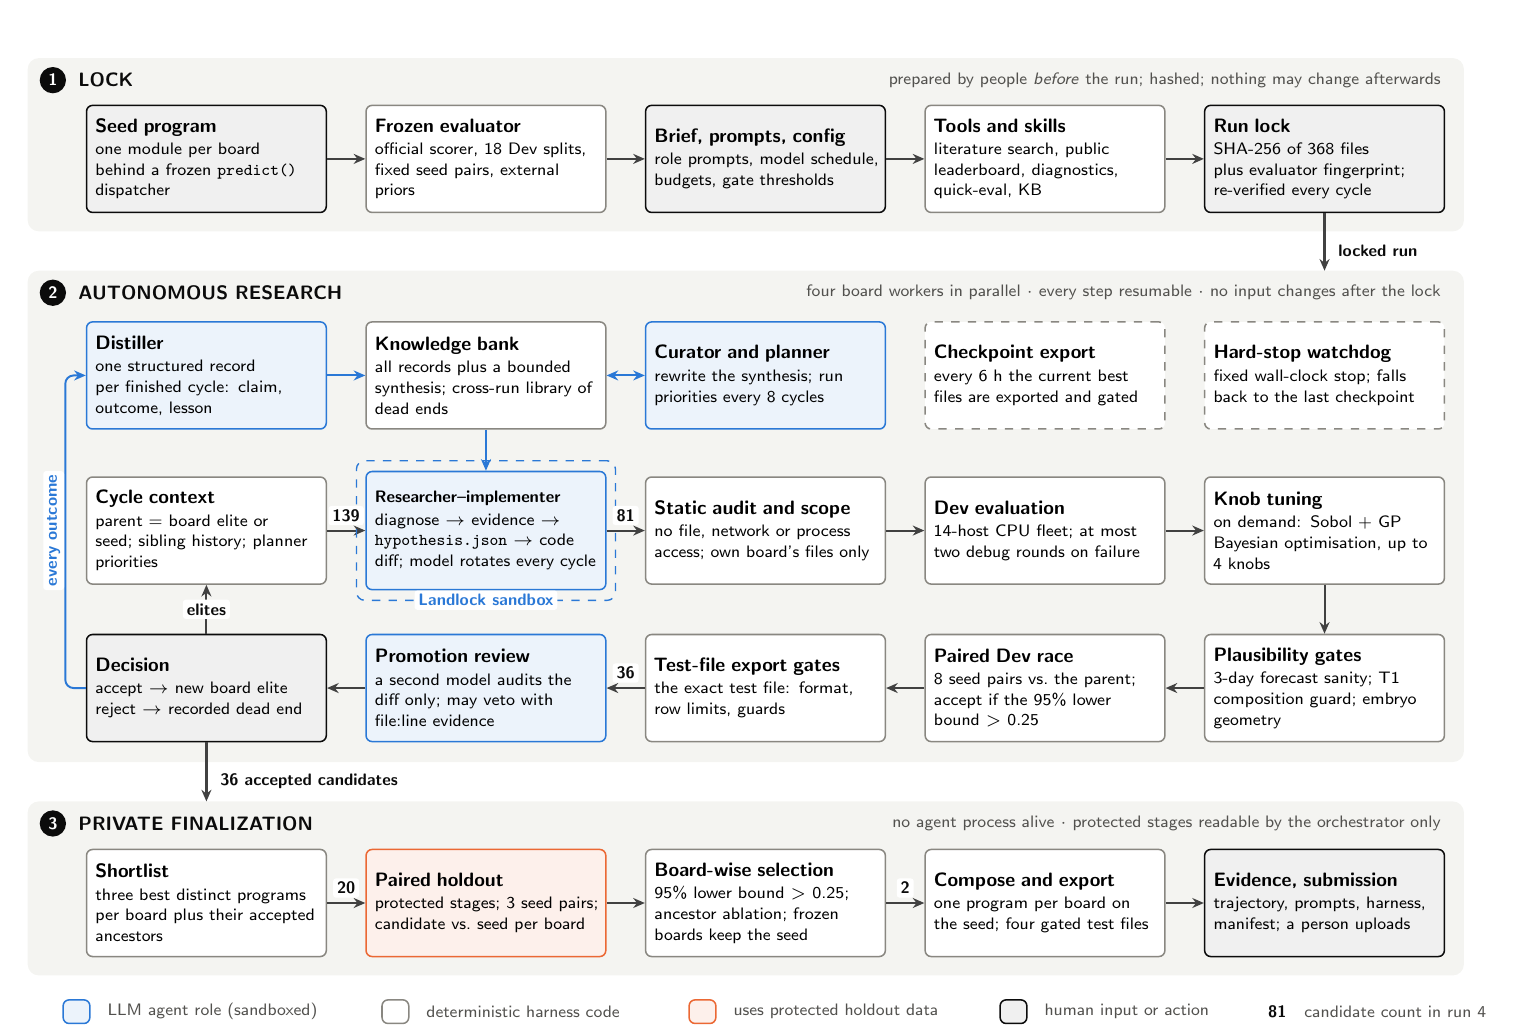
\begin{tikzpicture}[
    font=\sffamily\fontsize{6.3}{7.5}\selectfont,
    >={Stealth[length=4.2pt,width=3.6pt]},
    blk/.style={draw=#1, line width=0.55pt, rounded corners=2.2pt, fill=white, align=left,
                text width=2.82cm, minimum height=1.36cm, inner xsep=3.2pt, inner ysep=2.6pt,
                execute at begin node={\hyphenpenalty=10000 \exhyphenpenalty=10000 }},
    det/.style={blk=asmuted},
    llm/.style={blk=asblue, fill=asblue!9},
    prot/.style={blk=asorange, fill=asorange!10},
    hum/.style={blk=asink, fill=asink!6},
    svc/.style={blk=asmuted, dashed, fill=white},
    flow/.style={->, line width=0.7pt, draw=asink!78},
    feed/.style={->, line width=0.7pt, draw=asblue},
    lane/.style={fill=#1, rounded corners=4pt, draw=none},
    lanetitle/.style={font=\sffamily\bfseries\fontsize{7.2}{8}\selectfont, text=asink, anchor=west},
    lanenote/.style={font=\sffamily\fontsize{6.2}{7}\selectfont, text=asinktwo, anchor=east},
    tag/.style={font=\sffamily\bfseries\fontsize{5.8}{6.5}\selectfont, text=asink, fill=white, inner sep=1.4pt, rounded corners=1pt},
    num/.style={circle, fill=asink, text=white, font=\sffamily\bfseries\fontsize{6.5}{7}\selectfont, inner sep=1.3pt, minimum size=9.5pt}]
  \newcommand{\hd}[1]{{\bfseries\fontsize{6.9}{7.8}\selectfont #1}\\[0.6pt]}
  \def\xa{1.65}\def\xb{5.20}\def\xc{8.75}\def\xd{12.30}\def\xe{15.85}
  \def\yA{0}\def\yK{-2.75}\def\yR{-4.72}\def\yS{-6.72}\def\yC{-9.45}

  % ------------------------------------------------------------------ lane backgrounds
  \begin{scope}[on background layer]
    \fill[lane=aslane] (-0.62,1.28) rectangle (17.62,-0.92);
    \fill[lane=aslane] (-0.62,-1.42) rectangle (17.62,-7.66);
    \fill[lane=aslane] (-0.62,-8.16) rectangle (17.62,-10.37);
  \end{scope}
  \node[num] at (-0.30,1.00) {1};
  \node[lanetitle] at (-0.10,1.00) {LOCK};
  \node[lanenote] at (17.45,1.00) {prepared by people \emph{before} the run; hashed; nothing may change afterwards};
  \node[num] at (-0.30,-1.70) {2};
  \node[lanetitle] at (-0.10,-1.70) {AUTONOMOUS RESEARCH};
  \node[lanenote] at (17.45,-1.70) {four board workers in parallel $\cdot$ every step resumable $\cdot$ no input changes after the lock};
  \node[num] at (-0.30,-8.44) {3};
  \node[lanetitle] at (-0.10,-8.44) {PRIVATE FINALIZATION};
  \node[lanenote] at (17.45,-8.44) {no agent process alive $\cdot$ protected stages readable by the orchestrator only};

  % ------------------------------------------------------------------ lane 1: lock
  \node[hum]  (seed) at (\xa,\yA) {\hd{Seed program}one module per board behind a frozen \texttt{predict()} dispatcher};
  \node[det]  (eval) at (\xb,\yA) {\hd{Frozen evaluator}official scorer, 18 Dev splits, fixed seed pairs, external priors};
  \node[hum]  (brief) at (\xc,\yA) {\hd{Brief, prompts, config}role prompts, model schedule, budgets, gate thresholds};
  \node[det]  (tools) at (\xd,\yA) {\hd{Tools and skills}literature search, public leaderboard, diagnostics, quick-eval, KB};
  \node[det, fill=asink!6, draw=asink] (lock) at (\xe,\yA) {\hd{Run lock}SHA-256 of 368 files plus evaluator fingerprint; re-verified every cycle};
  \draw[flow] (seed) -- (eval);
  \draw[flow] (eval) -- (brief);
  \draw[flow] (brief) -- (tools);
  \draw[flow] (tools) -- (lock);

  % ------------------------------------------------------------------ lane 2, row K: memory and services
  \node[llm]  (dist) at (\xa,\yK) {\hd{Distiller}one structured record per finished cycle: claim, outcome, lesson};
  \node[det]  (kb)   at (\xb,\yK) {\hd{Knowledge bank}all records plus a bounded synthesis; cross-run library of dead ends};
  \node[llm]  (cur)  at (\xc,\yK) {\hd{Curator and planner}rewrite the synthesis; run priorities every 8 cycles};
  \node[svc]  (chk)  at (\xd,\yK) {\hd{Checkpoint export}every 6 h the current best files are exported and gated};
  \node[svc]  (stop) at (\xe,\yK) {\hd{Hard-stop watchdog}fixed wall-clock stop; falls back to the last checkpoint};
  \draw[feed] (dist) -- (kb);
  \draw[feed, <->] (kb) -- (cur);

  % ------------------------------------------------------------------ lane 2, row R: propose and measure
  \node[det]  (par)  at (\xa,\yR) {\hd{Cycle context}parent = board elite or seed; sibling history; planner priorities};
  \node[llm, minimum height=1.5cm]  (res)  at (\xb,\yR) {\hd{\mbox{\fontsize{6.5}{7.5}\selectfont Researcher--implementer}}diagnose $\rightarrow$ evidence $\rightarrow$ \texttt{hypothesis.json} $\rightarrow$ code diff; model rotates every cycle};
  \node[det]  (aud)  at (\xc,\yR) {\hd{Static audit and scope}no file, network or process access; own board's files only};
  \node[det]  (dev)  at (\xd,\yR) {\hd{Dev evaluation}14-host CPU fleet; at most two debug rounds on failure};
  \node[det]  (tune) at (\xe,\yR) {\hd{Knob tuning}on demand: Sobol + GP Bayesian optimisation, up to 4 knobs};
  \draw[flow] (par) -- (res);
  \draw[flow] (res) -- (aud);
  \draw[flow] (aud) -- (dev);
  \draw[flow] (dev) -- (tune);
  \draw[feed] (kb) -- (res);
  % sandbox boundary around the researcher
  \node[draw=asblue, dashed, line width=0.5pt, rounded corners=3pt, inner xsep=3.2pt, inner ysep=3.6pt, fit=(res)] (sbx) {};
  \node[tag, text=asblue] at ([yshift=0.3pt]sbx.south) {Landlock sandbox};

  % ------------------------------------------------------------------ lane 2, row S: decide
  \node[det]  (gate) at (\xe,\yS) {\hd{Plausibility gates}3-day forecast sanity; T1 composition guard; embryo geometry};
  \node[det]  (race) at (\xd,\yS) {\hd{Paired Dev race}8 seed pairs vs.\ the parent; accept if the 95\% lower bound $>$ 0.25};
  \node[det]  (exp)  at (\xc,\yS) {\hd{Test-file export gates}the exact test file: format, row limits, guards};
  \node[llm]  (rev)  at (\xb,\yS) {\hd{Promotion review}a second model audits the diff only; may veto with file:line evidence};
  \node[det, fill=asink!6, draw=asink] (dec) at (\xa,\yS) {\hd{Decision}accept $\rightarrow$ new board elite\\reject $\rightarrow$ recorded dead end};
  \draw[flow] (tune) -- (gate);
  \draw[flow] (gate) -- (race);
  \draw[flow] (race) -- (exp);
  \draw[flow] (exp) -- (rev);
  \draw[flow] (rev) -- (dec);
  \draw[flow] (dec) -- node[tag, pos=0.5] {elites} (par);
  % every outcome -> distiller (outer left channel)
  \draw[feed, rounded corners=3pt] (dec.west) -- ++(-0.26,0) |- (dist.west);
  \node[tag, text=asblue, rotate=90] at (-0.29,-4.72) {every outcome};

  % ------------------------------------------------------------------ lane 3: finalization
  \node[det]  (short) at (\xa,\yC) {\hd{Shortlist}three best distinct programs per board plus their accepted ancestors};
  \node[prot] (hold)  at (\xb,\yC) {\hd{Paired holdout}protected stages; 3 seed pairs; candidate vs.\ seed per board};
  \node[det]  (sel)   at (\xc,\yC) {\hd{Board-wise selection}95\% lower bound $>$ 0.25; ancestor ablation; frozen boards keep the seed};
  \node[det]  (comp)  at (\xd,\yC) {\hd{Compose and export}one program per board on the seed; four gated test files};
  \node[hum]  (evi)   at (\xe,\yC) {\hd{Evidence, submission}trajectory, prompts, harness, manifest; a person uploads};
  \draw[flow] (short) -- (hold);
  \draw[flow] (hold) -- (sel);
  \draw[flow] (sel) -- (comp);
  \draw[flow] (comp) -- (evi);

  % ------------------------------------------------------------------ lane-to-lane arrows with counts
  \draw[flow, line width=0.9pt] (lock.south) -- (\xe,-1.42);
  \node[tag, anchor=west] at (\xe+0.12,-1.17) {locked run};
  \draw[flow, line width=0.9pt] (dec.south) -- (\xa,-8.16);
  \node[tag, anchor=west] at (\xa+0.12,-7.91) {36 accepted candidates};

  % counts along the research loop (Normandy run)
  \node[tag] at ($(par.east)!0.5!(res.west)+(0,0.19)$) {139};
  \node[tag] at ($(res.east)!0.5!(aud.west)+(0,0.19)$) {81};
  \node[tag] at ($(exp.west)!0.5!(rev.east)+(0,0.19)$) {36};
  \node[tag] at ($(short.east)!0.5!(hold.west)+(0,0.19)$) {20};
  \node[tag] at ($(sel.east)!0.5!(comp.west)+(0,0.19)$) {2};

  % ------------------------------------------------------------------ legend
  \begin{scope}[shift={(0,-10.83)}]
    \node[llm, minimum height=0.30cm, text width=0.34cm, inner sep=0pt] (l1) at (0.0,0) {};
    \node[anchor=west, text=asinktwo] at (0.27,0) {LLM agent role (sandboxed)};
    \node[det, minimum height=0.30cm, text width=0.34cm, inner sep=0pt] at (4.05,0) {};
    \node[anchor=west, text=asinktwo] at (4.32,0) {deterministic harness code};
    \node[prot, minimum height=0.30cm, text width=0.34cm, inner sep=0pt] at (7.95,0) {};
    \node[anchor=west, text=asinktwo] at (8.22,0) {uses protected holdout data};
    \node[hum, minimum height=0.30cm, text width=0.34cm, inner sep=0pt] at (11.9,0) {};
    \node[anchor=west, text=asinktwo] at (12.17,0) {human input or action};
    \node[tag] at (15.25,0) {81};
    \node[anchor=west, text=asinktwo] at (15.47,0) {candidate count in run~4};
  \end{scope}
\end{tikzpicture}
}
\caption{\textbf{Architecture of AgenticScientist.} (1)~People prepare the seed program, frozen evaluator, prompts
and configuration; all 368 files are hashed into a lock. (2)~Board workers run research cycles in parallel after the lock: a sandboxed researcher model writes a hypothesis and a code diff, and the harness audits, evaluates,
tunes, gates and races the candidate against its parent before a second model reviews the diff. (3)~After research ends, a separate process with access
to protected stages re-scores the shortlisted programs and composes the final program board by board. Small numbers
give the count of candidates that reached each step in run~4.}
\label{fig:arch}
\end{figure*}

\section{Problem setting}

\begin{table}[t]
\caption{\textbf{Hidden test boards.} Inputs are the stages a program receives at test time.}
\label{tab:tasks}
\sffamily\fontsize{7.3}{9}\selectfont
\begin{tabularx}{\columnwidth}{@{}L{1.25cm}L{2.55cm}L{1.55cm}Y@{}}
\toprule
\textbf{Board} & \textbf{Inputs} & \textbf{Target} & \textbf{Output} \\
\midrule
T1 temporal & snRNA-seq E8.5, E9.5, E10.5 & E12.5 heart chambers & $\le$5,118 cells, expression \\
T2 heart & spatial E8.25--E10.5 (5~stages) & E12.5 dissected heart & $\le$25,179 cells, expression + 3D \\
T2 embryo & spatial E7.5, E8.0 & E7.75 whole embryo & $\le$5,000 cells, expression + 3D \\
T3 knockout & wild type E8.0--E8.75 (4~stages) & E8.75 $\beta$-catenin (\emph{Ctnnb1}) mutant & $\le$7,449 cells, expression + 3D \\
\bottomrule
\end{tabularx}
\end{table}

\paragraph{Tasks} The challenge scores four hidden test boards (Table~\ref{tab:tasks}). A submission is a set of
predicted cells: an expression matrix over a fixed gene panel and, for Tasks~2 and~3, a 3D coordinate per cell. A
board score is a weighted mean of metric skills on which a floor model (a copy of the last input stage, or of the
matched wild type) scores 50 and the attainable ceiling scores 100 \cite{vec2026}. Expression metrics are
differential-expression recovery (DE), its direction, a maximum mean discrepancy in a PCA space of the target (MMD)
\cite{gretton2012kernel} and a gene-pair variogram. Spatial boards add shape, occupancy, scale and neighbourhood
terms, and Task~3 a severity slope. The total is
\begin{equation}
S = S_{\mathrm{T1}} + \tfrac{1}{2}\left(S_{\mathrm{heart}} + S_{\mathrm{embryo}}\right) + S_{\mathrm{T3}}. \label{eq:total}
\end{equation}

\paragraph{Why local validation is hard} The released data stop at E10.5 for the heart and at E8.0 for the embryo.
Both extrapolation targets are dissected organs at E12.5, whereas the released sections contain surrounding tissue.
The knockout gene of the test is absent from the measured panel, and only one other knockout is released. Every local
split is therefore a proxy that differs from the test in horizon, protocol or gene, and a team may make only two
official submissions per board.

\paragraph{Agent-track constraints} Once a run starts, its prompts, harness, models, tools and budget are fixed, and
a person may not steer it on intermediate results. Choosing which \emph{completed} run to submit remains a human
decision, and everything is permitted before the lock \cite{vec2026}. Human judgement therefore enters through the
contents of the lock, and all selection inside a run is automatic.

% =====================================================================================================================
\section{The AgenticScientist harness}

Figure~\ref{fig:arch} gives the design. The harness is about 7,000 lines of Python around the command-line agents of
four vendors. Its evaluation core grew out of a program-evolution pipeline \cite{lange2025shinka} and its
orchestrator out of a predecessor harness (Section~\ref{sec:pre}).

\subsection{Lock and program contract}

A lock file holds the SHA-256 digest of every file that can influence a run: the seed program, the evaluator and its
splits, prompts, tools and the configuration with its budgets and thresholds. The orchestrator verifies it at
start-up, at the beginning of every cycle and at finalization, and refuses to continue on a mismatch. The object
under research is a \emph{program}, not a set of weights. It exposes one function,
\code{predict(board, inputs, times, target\_time, context)}, with one group of module files per board, and may not
touch the file system, network or other processes. Because the board groups are disjoint, programs found by
different workers can be composed by copying groups onto the seed.

\subsection{The research cycle}

Each worker owns one board. In a cycle it picks a parent among the board's four best accepted programs and assembles
a prompt from the brief, the parent's per-split and per-metric development scores, a curated knowledge synthesis and
its last five outcomes. A single model session then collects test-side evidence from the public leaderboard, whose
entry names often describe a recipe, runs diagnostics on the parent, writes \code{hypothesis.json} with a falsifiable
claim and the metrics expected to move, and implements the change in a copy of the parent. The predecessor harness
separated ideation and implementation; we merged them because hand-offs between models lost design intent.

The researcher model rotates every cycle over Claude Fable~5.2, GPT-6.2~Sol and Gemini~4~Neon. Subscription quotas
are the binding resource in a day-long run, so the orchestrator detects rate-limit signatures, marks the provider as
limited and reroutes the role along a fixed fallback chain (Claude Opus~5.5, Gemini~4~Neon, DeepSeek~v4.1~Flash,
GPT-6~Luna). Every agent session runs inside a Linux Landlock allowlist \cite{salaun2017landlock}: read-only access
to the repository, released stages and external priors, read-write access to its own cycle directory, and no access
to the protected stages.

A frozen evaluator scores each candidate on 18 development splits (\dev) built from released stages (Table~\ref{tab:data}) with the official scorer, aggregated as in Eq.~\ref{eq:total}. Numeric knobs that a candidate declares (at most four per board) are tuned by the harness with Bayesian optimisation \cite{snoek2012practical} on a disjoint seed pair, never by an agent. Every finished cycle is distilled into a structured record (claim, mechanism, outcome with statistics and a retry condition), and the records persist across runs in a library that agents can query.

\subsection{Paired racing, gates and review}

Programs sample cells and the scorer subsamples, so a candidate $c$ and its parent $p$ are evaluated on the same
(prediction seed, fit seed) pairs and compared through paired differences, as in racing algorithms
\cite{birattari2002racing}. With mean $\bar d$ and standard deviation $s$ of the differences over $n$ pairs, the
one-sided 95\% bounds are
\begin{equation}
\mathrm{LB},\,\mathrm{UB} = \bar d \mp t_{0.95,\,n-1}\, s/\sqrt{n}. \label{eq:lb}
\end{equation}
A screen on three scoring seeds rejects clear losses; survivors are raced on eight further pairs. A candidate is
accepted if $\mathrm{LB}>0.25$, and rejected if any board drops significantly. The two spatial boards must clear
their own margin, and \emph{condition rules} forbid trading one target for another: no group of splits that shares a
stage, protocol or knockout gene may lose more than 0.25 on average.

Three gates run without ground truth: a plausibility check that forecasts three days ahead in the test configuration,
a T1 composition guard (no more blood-like cells than the last input and at least 0.9 times its cardiomyocyte share)
and an embryo geometry gate. A candidate that wins the race is finally audited by a different model, which sees only
the diff, the hypothesis and the race statistics. It may veto for a rule violation, a breakage of the test code path
or a diff that does something materially different from the hypothesis, but not for style or doubts about effect
size.

\subsection{Holdout-calibrated selection}
\label{sec:final}

Research ends at a fixed wall-clock time, and selection runs after every agent session has exited. For each board we
withheld the local targets that most resemble the test (Table~\ref{tab:data}): a two-day dissected-heart forecast
from an external perinatal atlas for T1, the two-day jump to the validation-phase E10.5 heart, and the
validation-phase E7.5 embryo. Agents can neither read these files nor see scores computed on them.

For each board the three best distinct accepted programs by development score are shortlisted with their accepted ancestors, and each is scored against the seed on three fresh seed pairs. A change is eligible if its paired lower bound (Eq.~\ref{eq:lb}, $n=3$) exceeds 0.25. Among eligible programs the one with the largest mean gain is taken, unless an accepted ancestor reaches within 0.25 of it, in which case the simpler ancestor is preferred. Boards without an eligible change keep the seed. Where local splits cannot order programs of known test score, the board is excluded from research: before run~4 a \emph{calibration ladder} of our earlier entries and of replicated public recipes showed that the T3 splits ranked real-cell delay mixtures below the matched wild type, the reverse of the test, so T3 was frozen at its seed. A watchdog enforces a hard stop before the deadline and falls back to the last gated checkpoint.

\begin{table*}[t]
\caption{\textbf{What was fitted on what.} No neural network is trained: every program is a non-parametric sampler
that is fitted at prediction time on the stages it is given. The table lists the data behind each board's final
program, the development splits on which agents and the tuner chose mechanisms and constants, and the protected
holdout used only at finalization. External sources are restricted to stages outside the challenge's held-out window
and exclude perturbation data for \emph{Gata4}, \emph{Ctnnb1} and the Wnt pathway.}
\label{tab:data}
\sffamily\fontsize{7.2}{9}\selectfont
\begin{tabularx}{\textwidth}{@{}L{1.3cm}L{3.9cm}L{4.3cm}L{4.1cm}Y@{}}
\toprule
\textbf{Board} & \textbf{Data used by the final program at prediction time} & \textbf{External priors passed in
\code{context}} & \textbf{Development splits (visible to agents)} & \textbf{Protected holdout (finalization only)} \\
\midrule
T1 temporal & Cells of the supplied stages; the latest stage (E10.5) is the donor pool &
Qiu et al.\ atlas \cite{qiu2024timelapse}: Theiler stages 12--13 and 23--25 only (stages covering E9.5--E13.5 never
transferred) &
E8.5, E9.5 $\rightarrow$ E10.5 (validation stage): whole target and a composition-matched cardiac target &
Perinatal heart atlas \cite{feulner2024}: E14.5, E16.5 $\rightarrow$ E18.5 \\
T2 heart & Cells and coordinates of the supplied stages; the latest stage is the donor pool &
Perinatal heart atlas \cite{feulner2024}, E14.5 and E16.5 pseudobulk; Slide-seq heart atlas (GEO GSE282547), E14.5 and
E15.5 pucks only &
Seven splits from E8.25--E9.5: one-day and half-day jumps, whole-section and dissected-organ targets &
E8.25, E8.5 $\rightarrow$ E10.5 (validation stage), dissected-organ and spatial-region targets \\
T2 embryo & Cells and coordinates of the two bracketing stages & none read by the final program &
E6.75, E8.0 $\rightarrow$ E7.25; E7.25, E8.25 $\rightarrow$ E8.0 &
E7.25, E8.0 $\rightarrow$ E7.5 (validation stage) \\
T3 knockout & Wild-type cells and coordinates of the four supplied stages; no mutant data &
Gene Ontology annotations \cite{ashburner2000go} without mutant-phenotype evidence codes and without
\emph{Ctnnb1}/\emph{Gata4} citations; per-gene expression prior from wild-type atlas cells \cite{qiu2024timelapse} &
\emph{Gata4} (two replicates), \emph{Mab21l2}; external \emph{Hand2} \cite{desoysa2019} and \emph{Mef2c}
\cite{muncievasic2025} knockouts with matched wild type &
none in run~4 (board frozen at the seed) \\
\bottomrule
\end{tabularx}
\end{table*}

\subsection{The forecasting programs}
\label{sec:programs}

The harness is agnostic to the method inside \code{predict}. The programs converged on one principle: \emph{emit
measured cells and decide which ones}. Every large distributional score we observed, locally or on the public board,
came from selecting, re-weighting or relocating real cells rather than from generating expression profiles.

\paragraph{T1 (seed plus agent change \code{w3\_c02})} The forecast is 5,000 real E10.5 nuclei. A
chamber-conditioning step down-weights non-cardiac tissues to 5\% and holds blood at 0.8 times its last-input share,
cardiac lineages keep their latest-stage masses, and a maturity tilt chooses which cells of each lineage are
emitted. Expression is then continued along an anchor direction from a public atlas \cite{qiu2024timelapse}. The
agent change replaced a single whole-embryo direction, which is confounded by the fall in cardiomyocyte share
between atlas stages, with lineage-specific directions.

\paragraph{T2 heart (seed plus four stacked agent changes, \code{w1\_c38})} The forecast is 25,179 real organ-resident E10.5 cells: cardiac labels including epicardium, plus vessel and pericardial cells attached to cardiac tissue. Expression is offset towards a fetal pseudobulk \cite{feulner2024} and the organ's radius grows towards a fixed envelope. The agents added a compartment-wise maturity tilt, a placement stack replicated from public recipes, a detection-prevalence correction and a decelerating (Gompertz) growth law.

\paragraph{T2 embryo (seed)} The forecast keeps the cells and positions of the nearer bracketing embryo, transplants
expression from local fields of the other bracket and rescales each imaging axis to the interpolated spread.

\paragraph{T3 (seed, frozen)} A gene-ontology gate classifies the knocked-out gene as a broad signalling regulator
or a narrow module. For the former the forecast is a developmental delay made only of measured wild-type cells: the
population 2.3 sampling intervals before the target, mixed from the two supplied stages that bracket it (2,235 E8.0
and 5,214 E8.25 cells for the test). The constant 2.3 was read from the names of public leaderboard entries, which
the rules allow.

% =====================================================================================================================
\section{Results}

\subsection{Predecessor experiments}
\label{sec:pre}

The selection rule was arrived at through failures. Before the four runs reported below we worked in a separate
repository, first by hand and then with an earlier harness in which a frontier model proposed a change, an
inexpensive model implemented it, and the program with the highest held-out proxy was taken at the end.

Learned generators were tested first, in 44 development runs with 1,060 paired metric evaluations: a conditional
variational autoencoder and a latent neural flow for T1, and state-flow models and a spatial hurdle autoencoder for
the heart. They did not survive a second backtest. Heart state-flow models gained 1.9 to 3.9 points on the earlier
of two backtests and lost 0.4 to 4.1 on the later one.

Eight locked runs followed: five short ones (108 cycles, 41 accepted changes) and three day-long ones named Turing
(58 cycles, 27 accepted), Enigma (59, 6) and Waddington (76, 20). Turing was the first to compare each board with
the seed on protected stages, and all six heart and embryo winners that it re-scored lost. The embryo programs stood
3.4 to 4.8 points above the seed on \dev{} and 3.8 to 4.9 below it on the protected stage; the heart programs stood
5.0 to 5.5 above and 0.3 to 1.6 below. The spatial-board margin, the condition rules and a final selection on unseen
stages were written in response, and under them Enigma accepted 6 of 59 cycles.

T1 had no protected stage in these two runs, and its development score rose from 59.3 to 70.3. The only T1
development target was E10.5, which is an input at test time, and the agents had fitted its composition: the selected
programs emitted 22\% and 28\% blood-like cells, against at most 17.5\% in the E10.5 chamber population. On the
hidden test the order was reversed. A hand-built sampler, more than 20 points below these programs on the development
split, scored well above them. The composition guard and the external T1 holdout follow from this result. Waddington
then ran every role on GPT-6.2~Sol. By that time no local check ordered the T1, heart or embryo programs of known
test order correctly, so its finalization could promote only a T3 change that beat a test-scored reference. None
did, and the run exported nothing. Seed~1 was assembled by people from this phase; the chamber-conditioning rule of
its T1 program was first written by an agent in one of the short runs.

\subsection{Four locked runs}

\begin{table}[t]
\caption{\textbf{The four locked runs.} ``Holdout-selected'' lists board changes promoted by the finalization rule.
Run~3 exported the files that run~2 had selected. Cost is the API-equivalent cost reported by one vendor's client
only.}
\label{tab:runs}
\sffamily\fontsize{7.2}{9}\selectfont
\begin{tabularx}{\columnwidth}{@{}Y r r r r@{}}
\toprule
 & \textbf{Run 1} & \textbf{Run 2} & \textbf{Run 3} & \textbf{Run 4} \\
 & & & \textbf{D-Day} & \textbf{Normandy} \\
\midrule
Research time (h) & 10.6 & 2.9 & 14.3 & 26.7 \\
Research cycles & 77 & 14 & 68 & 139 \\
\quad accepted on \dev & 28 & 3 & 21 & 36 \\
\quad vetoed in review & 19 & 1 & 13 & 0 \\
\quad no candidate & 8 & 4 & 14 & 58 \\
Agent calls & 331 & 53 & 386 & 881 \\
\quad on a substitute model (\%) & 39 & 52 & 75 & 75 \\
Re-scored on holdout & 6 & 3 & 12 & 20 \\
Holdout-selected & none & heart & none & T1, heart \\
Metered cost (US\$) & 31 & 9 & 39 & 310 \\
Research ended by & -- & operator & operator & schedule \\
Files submitted & no & \multicolumn{2}{c}{yes (identical files)} & yes \\
\bottomrule
\end{tabularx}
\end{table}

We ran the present harness four times, each time with a new lock (Table~\ref{tab:runs}). Between runs, people
analysed the \emph{completed} run and changed the seed, the splits and the gates; within a run nothing changed. The
runs form a chain (Fig.~\ref{fig:lineage}). Run~1 had a protected holdout for the embryo board only, so it composed
the development-best T1, heart and T3 programs with the embryo seed. That composition, with fifteen hand-edited
lines, became the seed of run~2, whose finalization added one heart change. Run~3 (``D-Day'') was seeded with the
selection of run~2 byte for byte and produced our first official submission. People then redesigned the seed from the
per-metric test feedback, and run~4 (``Normandy'') produced the second submission.

\begin{figure*}[t] \centering \resizebox{\textwidth}{!}{% Provenance of the submitted files across the four locked runs (TikZ). Included by main.tex; colours are defined there.
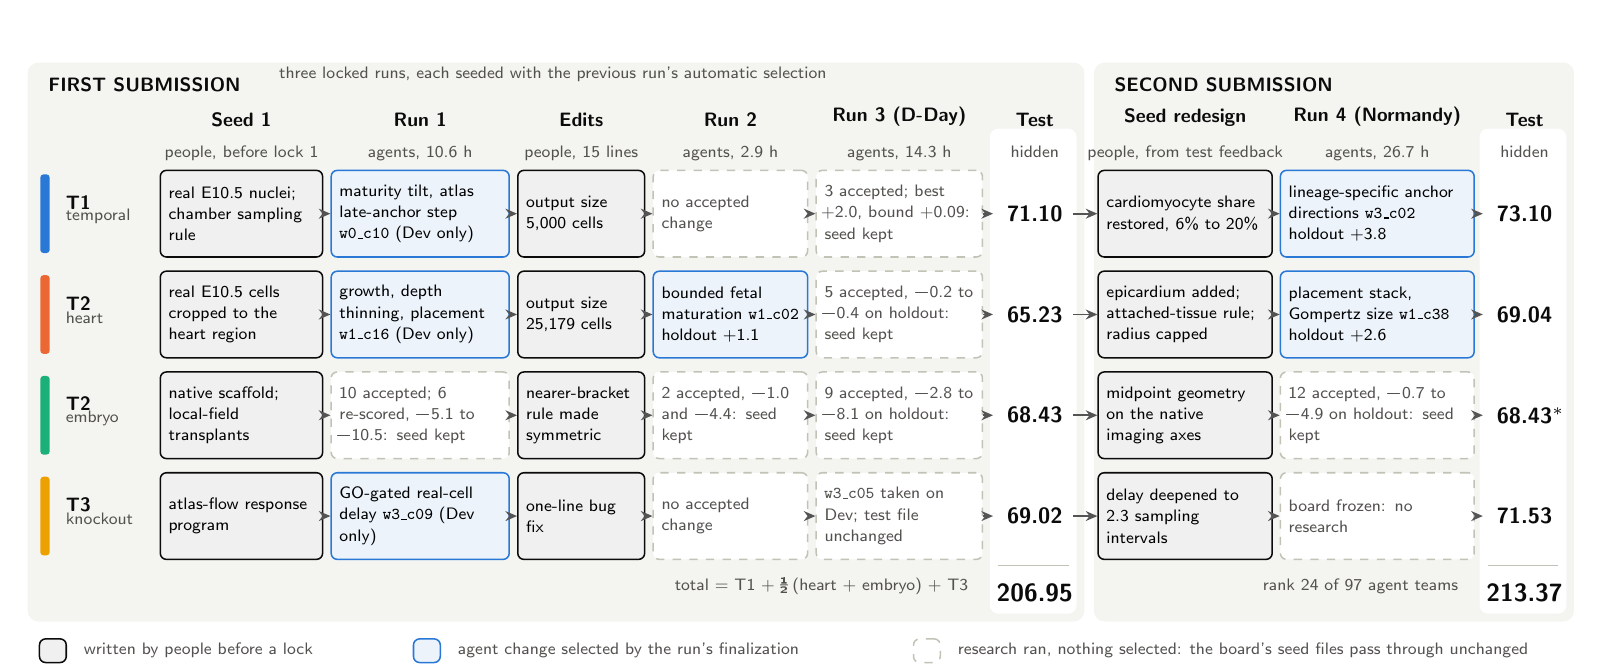
\begin{tikzpicture}[
    font=\sffamily\fontsize{6.4}{7.7}\selectfont,
    >={Stealth[length=4.2pt,width=3.6pt]},
    cell/.style={draw=#1, line width=0.55pt, rounded corners=2.2pt, fill=white, align=left, minimum height=1.1cm,
                 inner xsep=3pt, inner ysep=2.4pt, anchor=center,
                 execute at begin node={\hyphenpenalty=10000 \exhyphenpenalty=10000 \raggedright}},
    hum/.style={cell=asink, fill=asink!6},
    agt/.style={cell=asblue, fill=asblue!9},
    non/.style={cell=asrule, dashed, text=asinktwo},
    tst/.style={font=\sffamily\bfseries\fontsize{8}{9}\selectfont, text=asink, anchor=center},
    hdr/.style={font=\sffamily\bfseries\fontsize{6.9}{7.8}\selectfont, text=asink, anchor=south, align=center},
    sub/.style={font=\sffamily\fontsize{6}{7}\selectfont, text=asinktwo, anchor=north, align=center},
    brd/.style={font=\sffamily\bfseries\fontsize{6.9}{7.8}\selectfont, text=asink, anchor=west},
    tag/.style={font=\sffamily\bfseries\fontsize{5.8}{6.5}\selectfont, text=asink, fill=white, inner sep=1.4pt, rounded corners=1pt}]
  \newcommand{\id}[1]{{\bfseries\ttfamily\fontsize{6.1}{7.4}\selectfont #1}}
  % column centres and widths
  \def\xa{2.595}\def\cwa{1.85}   % seed 1
  \def\xb{4.865}\def\cwb{2.05}   % run 1
  \def\xc{6.910}\def\cwc{1.40}   % pre-lock edits
  \def\xd{8.805}\def\cwd{1.75}   % run 2
  \def\xe{10.95}\def\cwe{1.90}   % run 3
  \def\xf{12.67}                 % test 1
  \def\xg{14.58}\def\cwg{2.00}   % seed redesign
  \def\xh{17.02}\def\cwh{2.25}   % run 4
  \def\xj{18.89}                 % test 2
  \def\ya{0}\def\yb{-1.28}\def\yc{-2.56}\def\yd{-3.84}\def\yt{-4.82}

  % ------------------------------------------------------------------ backgrounds
  \begin{scope}[on background layer]
    \fill[aslane, rounded corners=4pt] (-0.12,1.92) rectangle (13.30,-5.18);
    \fill[aslane, rounded corners=4pt] (13.42,1.92) rectangle (19.52,-5.18);
    \fill[white, rounded corners=3pt] (12.10,1.08) rectangle (13.20,-5.08);
    \fill[white, rounded corners=3pt] (18.32,1.08) rectangle (19.42,-5.08);
  \end{scope}
  \node[brd, anchor=west] at (0.02,1.64) {FIRST SUBMISSION};
  \node[sub, anchor=west] at (2.95,1.765) {three locked runs, each seeded with the previous run's automatic selection};
  \node[brd, anchor=west] at (13.56,1.64) {SECOND SUBMISSION};

  % ------------------------------------------------------------------ column headers
  \node[hdr] at (\xa,0.98) {Seed 1};            \node[sub] at (\xa,0.98) {people, before lock 1};
  \node[hdr] at (\xb,0.98) {Run 1};             \node[sub] at (\xb,0.98) {agents, 10.6 h};
  \node[hdr] at (\xc,0.98) {Edits};             \node[sub] at (\xc,0.98) {people, 15 lines};
  \node[hdr] at (\xd,0.98) {Run 2};             \node[sub] at (\xd,0.98) {agents, 2.9 h};
  \node[hdr] at (\xe,0.98) {Run 3 (D-Day)};     \node[sub] at (\xe,0.98) {agents, 14.3 h};
  \node[hdr] at (\xf,0.98) {Test};              \node[sub] at (\xf,0.98) {hidden};
  \node[hdr] at (\xg,0.98) {Seed redesign};     \node[sub] at (\xg,0.98) {people, from test feedback};
  \node[hdr] at (\xh,0.98) {Run 4 (Normandy)};  \node[sub] at (\xh,0.98) {agents, 26.7 h};
  \node[hdr] at (\xj,0.98) {Test};              \node[sub] at (\xj,0.98) {hidden};

  % ------------------------------------------------------------------ row labels
  \foreach \y/\c/\t/\s in {\ya/asblue/T1/temporal, \yb/asorange/T2/heart, \yc/asaqua/T2/embryo, \yd/asyellow/T3/knockout} {
    \fill[\c, rounded corners=1.2pt] (0.04,\y-0.5) rectangle (0.16,\y+0.5);
    \node[brd] at (0.24,\y+0.14) {\t};
    \node[sub, anchor=west] at (0.24,\y-0.04) {\s};
  }

  % ------------------------------------------------------------------ T1
  \node[hum, text width=\cwa cm] (a1) at (\xa,\ya) {real E10.5 nuclei; chamber sampling rule};
  \node[agt, text width=\cwb cm] (b1) at (\xb,\ya) {maturity tilt, atlas late-anchor step \id{w0\_c10} (Dev only)};
  \node[hum, text width=\cwc cm] (c1) at (\xc,\ya) {output size 5,000 cells};
  \node[non, text width=\cwd cm] (d1) at (\xd,\ya) {no accepted change};
  \node[non, text width=\cwe cm] (e1) at (\xe,\ya) {3 accepted; best +2.0, bound +0.09: seed kept};
  \node[tst] at (\xf,\ya) {71.10};
  \node[hum, text width=\cwg cm] (g1) at (\xg,\ya) {cardiomyocyte share restored, 6\% to 20\%};
  \node[agt, text width=\cwh cm] (h1) at (\xh,\ya) {lineage-specific anchor directions \id{w3\_c02}\\holdout +3.8};
  \node[tst] at (\xj,\ya) {73.10};

  % ------------------------------------------------------------------ heart
  \node[hum, text width=\cwa cm] (a2) at (\xa,\yb) {real E10.5 cells cropped to the heart region};
  \node[agt, text width=\cwb cm] (b2) at (\xb,\yb) {growth, depth thinning, placement \id{w1\_c16} (Dev only)};
  \node[hum, text width=\cwc cm] (c2) at (\xc,\yb) {output size 25,179 cells};
  \node[agt, text width=\cwd cm] (d2) at (\xd,\yb) {bounded fetal maturation \id{w1\_c02}\\holdout +1.1};
  \node[non, text width=\cwe cm] (e2) at (\xe,\yb) {5 accepted, \textminus0.2 to \textminus0.4 on holdout: seed kept};
  \node[tst] at (\xf,\yb) {65.23};
  \node[hum, text width=\cwg cm] (g2) at (\xg,\yb) {epicardium added; attached-tissue rule; radius capped};
  \node[agt, text width=\cwh cm] (h2) at (\xh,\yb) {placement stack, Gompertz size \id{w1\_c38}\\holdout +2.6};
  \node[tst] at (\xj,\yb) {69.04};

  % ------------------------------------------------------------------ embryo
  \node[hum, text width=\cwa cm] (a3) at (\xa,\yc) {native scaffold; local-field transplants};
  \node[non, text width=\cwb cm] (b3) at (\xb,\yc) {10 accepted; 6 re-scored, \textminus5.1 to \textminus10.5: seed kept};
  \node[hum, text width=\cwc cm] (c3) at (\xc,\yc) {nearer-bracket rule made symmetric};
  \node[non, text width=\cwd cm] (d3) at (\xd,\yc) {2 accepted, \textminus1.0 and \textminus4.4: seed kept};
  \node[non, text width=\cwe cm] (e3) at (\xe,\yc) {9 accepted, \textminus2.8 to \textminus8.1 on holdout: seed kept};
  \node[tst] at (\xf,\yc) {68.43};
  \node[hum, text width=\cwg cm] (g3) at (\xg,\yc) {midpoint geometry on the native imaging axes};
  \node[non, text width=\cwh cm] (h3) at (\xh,\yc) {12 accepted, \textminus0.7 to \textminus4.9 on holdout: seed kept};
  \node[tst] at (\xj,\yc) {68.43\rlap{$^{\ast}$}};

  % ------------------------------------------------------------------ T3
  \node[hum, text width=\cwa cm] (a4) at (\xa,\yd) {atlas-flow response program};
  \node[agt, text width=\cwb cm] (b4) at (\xb,\yd) {GO-gated real-cell delay \id{w3\_c09} (Dev only)};
  \node[hum, text width=\cwc cm] (c4) at (\xc,\yd) {one-line bug fix};
  \node[non, text width=\cwd cm] (d4) at (\xd,\yd) {no accepted change};
  \node[non, text width=\cwe cm] (e4) at (\xe,\yd) {\id{w3\_c05} taken on Dev; test file unchanged};
  \node[tst] at (\xf,\yd) {69.02};
  \node[hum, text width=\cwg cm] (g4) at (\xg,\yd) {delay deepened to 2.3 sampling intervals};
  \node[non, text width=\cwh cm] (h4) at (\xh,\yd) {board frozen: no research};
  \node[tst] at (\xj,\yd) {71.53};

  % ------------------------------------------------------------------ flow arrows
  \foreach \r in {1,2,3,4} {
    \draw[->, line width=0.6pt, draw=asink!70] (a\r) -- (b\r);
    \draw[->, line width=0.6pt, draw=asink!70] (b\r) -- (c\r);
    \draw[->, line width=0.6pt, draw=asink!70] (c\r) -- (d\r);
    \draw[->, line width=0.6pt, draw=asink!70] (d\r) -- (e\r);
    \draw[->, line width=0.6pt, draw=asink!70] (g\r) -- (h\r);
  }
  \foreach \y in {\ya,\yb,\yc,\yd} {
    \draw[->, line width=0.6pt, draw=asink!70] (\xe+0.5*\cwe+0.115,\y) -- (12.14,\y);
    \draw[->, line width=0.6pt, draw=asink!70] (13.16,\y) -- (\xg-0.5*\cwg-0.115,\y);
    \draw[->, line width=0.6pt, draw=asink!70] (\xh+0.5*\cwh+0.115,\y) -- (18.36,\y);
  }

  % ------------------------------------------------------------------ totals
  \draw[asrule, line width=0.5pt] (12.2,-4.47) -- (13.1,-4.47);
  \draw[asrule, line width=0.5pt] (18.42,-4.47) -- (19.32,-4.47);
  \node[tst, font=\sffamily\bfseries\fontsize{8.6}{9.5}\selectfont] at (\xf,\yt) {206.95};
  \node[tst, font=\sffamily\bfseries\fontsize{8.6}{9.5}\selectfont] at (\xj,\yt) {213.37};
  \node[sub, anchor=east] at (11.95,\yt+0.09) {total = T1 + \textonehalf\,(heart + embryo) + T3};
  \node[sub, anchor=east] at (18.17,\yt+0.09) {rank 24 of 97 agent teams};

  % ------------------------------------------------------------------ legend
  \begin{scope}[shift={(0.2,-5.55)}]
    \node[hum, minimum height=0.30cm, text width=0.34cm, inner sep=0pt] at (0,0) {};
    \node[anchor=west, text=asinktwo] at (0.27,0) {written by people before a lock};
    \node[agt, minimum height=0.30cm, text width=0.34cm, inner sep=0pt] at (4.75,0) {};
    \node[anchor=west, text=asinktwo] at (5.02,0) {agent change selected by the run's finalization};
    \node[non, minimum height=0.30cm, text width=0.34cm, inner sep=0pt] at (11.1,0) {};
    \node[anchor=west, text=asinktwo] at (11.37,0) {research ran, nothing selected: the board's seed files pass through unchanged};
  \end{scope}
\end{tikzpicture}
} \caption{\textbf{Provenance of the submitted files.} Each row follows one board's program through the four locked runs. Grey cells are code written by people before a lock, blue cells are agent changes that a run's finalization selected, and dashed cells are runs in which research took place but nothing was selected. Holdout values are paired gains over the seed of the same run; ``Dev only'' marks selections made in run~1 before a protected holdout existed for that board. The asterisk marks the team's standing embryo entry, which is the run-3 file.} \label{fig:lineage} \end{figure*}

\subsection{Run 3 (D-Day): a run that returned its seed}
\label{sec:dday}

In 14.3 hours run~3 finished 68 cycles with one worker per board. Fifty-four produced a candidate and 34 of those won the paired race. The reviewer vetoed 13, eleven because the diff did something materially different from the hypothesis, and 21 changes were accepted. Development scores rose on every board, the embryo score from 70.4 to 79.2.

Twelve accepted programs were re-scored on the protected stages. All five embryo programs lost 2.8 to 8.1 points,
all four heart programs lost 0.2 to 0.4, and two of three T1 programs lost 0.9. The third gained 2.0 on average, but
its lower bound over three seed pairs was $+0.09$, below the margin, and it was not promoted. The four exported files
were therefore identical, by SHA-256, to those of run~2. A composition of each board's development-best program
would instead have gained 8.6 development points and lost 1.7 on the holdout. An operator stopped the research phase
after 14.7 hours, before its scheduled end; selection, export and packaging were executed by the run's own
finalization code.

The files scored 206.95 on the hidden test (Table~\ref{tab:metrics}), and the per-metric feedback shaped the run-4
seed. On T1 the forecast contained 6\% cardiomyocytes where the chambers of the last input contain about 19\%. On the
heart board scale stood at 87.2 and the epicardium was missing from the organ definition. On the embryo board
occupancy was 3.7, the floor of a scaffold copied from the earlier bracket. On T3 a delay of 0.23 day stayed inside
the last sampling interval. The run also exposed a gap in the harness: three vetoed heart candidates were the only
ones that scored above the seed on the protected heart stage ($+1.1$ to $+1.2$), and a veto ends a candidate without
returning it to its author for repair.

\begin{table}[t]
\caption{\textbf{Hidden-test metric skills of both submissions} (50 = floor, 100 = ceiling). Dir, DE direction; Var,
variogram; Occ, occupancy; Nbr, neighbourhood MMD; Sev, severity slope. The embryo row is the team's standing
entry.}
\label{tab:metrics}
\sffamily\fontsize{6.9}{8.6}\selectfont\setlength{\tabcolsep}{2.6pt}
\begin{tabularx}{\columnwidth}{@{}Y r r r r r r r r r r@{}}
\toprule
 & \textbf{DE} & \textbf{Dir} & \textbf{MMD} & \textbf{Var} & \textbf{Shape} & \textbf{Occ} & \textbf{Scale} & \textbf{Nbr} & \textbf{Sev} & \textbf{Score} \\
\midrule
T1, run 3 & 68.0 & 78.5 & 66.4 & 72.8 & & & & & & \textbf{71.10} \\
T1, run 4 & 69.0 & 78.7 & 71.2 & 74.0 & & & & & & \textbf{73.10} \\
\addlinespace[2pt]
Heart, run 3 & 61.3 & 69.4 & 59.5 & 72.6 & 63.6 & 49.6 & 87.2 & 64.0 & & \textbf{65.23} \\
Heart, run 4 & 65.7 & 73.8 & 67.6 & 77.7 & 71.2 & 39.8 & 100.0 & 64.4 & & \textbf{69.04} \\
\addlinespace[2pt]
Embryo, run 3 & 65.1 & 73.4 & 79.2 & 59.0 & 63.3 & 3.7 & 99.8 & 77.8 & & \textbf{68.43} \\
\addlinespace[2pt]
T3, run 3 & 61.7 & 68.0 & 56.5 & 56.9 & & & & & 88.7 & \textbf{69.02} \\
T3, run 4 & 64.8 & 69.6 & 50.7 & 54.7 & & & & & 97.0 & \textbf{71.53} \\
\bottomrule
\end{tabularx}
\end{table}

\subsection{Run 4 (Normandy): development gains rarely transfer}

In 26.7 hours run~4 started 139 cycles with two T1 workers, one heart and one embryo worker. Eighty-one produced a
candidate and 36 were accepted. The 58 cycles without a candidate reflect provider limits: 512 of 880 logged agent
calls hit a rate limit and were rerouted. Development scores rose on all three boards, T1 from 69.2 to 78.8, heart
from 68.2 to 74.2 and embryo from 70.0 to 76.4.

Finalization re-scored 20 accepted programs against the seed (Fig.~\ref{fig:transfer}). On T1 the development-best
program had gained 9.5 points on \dev{} through four stacked edits and lost 9.1 on the two-day holdout. Its early
ancestor \code{w3\_c02}, with a \dev{} gain of 2.2, gained 3.8 on the holdout and was selected. On the heart board
the development-best program \code{w1\_c38} was also best on the holdout ($+2.6$) and was selected; most of that gain
came from its last edit, since its parent was neutral ($-0.1$). All nine embryo programs, with \dev{} gains of 0.6
to 6.4, lost 0.7 to 4.9 points, and the seed was kept.

Pooled over the four runs, 41 development winners were re-scored and five improved the holdout by more than the
margin (2 of 8 on T1, 3 of 11 on heart, 0 of 22 on embryo). Development gain predicted holdout gain positively only
on the heart board ($r=+0.41$); on T1 and embryo the correlation was strongly negative ($r=-0.89$ and $-0.83$). In
run~4 the selected composition raised the holdout proxy from 131.3 to 136.4 and the \dev{} proxy from 200.0 to 205.2.
A composition of each board's development-best program would have gained 15.7 \dev{} points and lost 10.1 holdout
points.

\begin{figure*}[t]
\centering
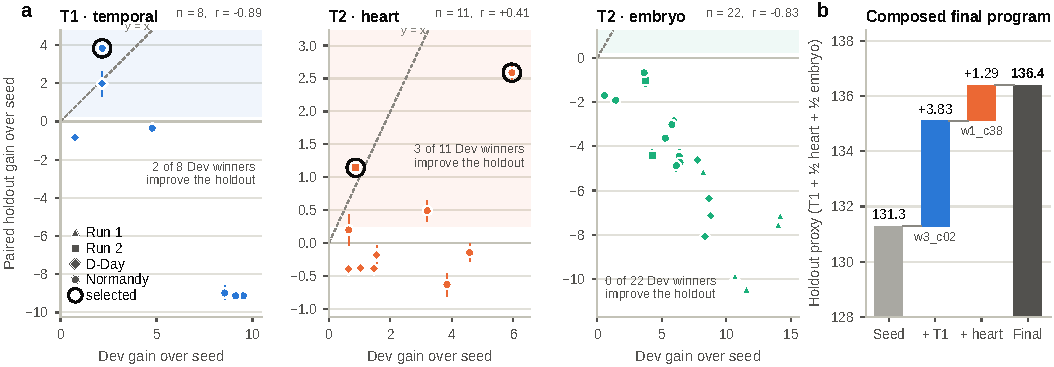
\includegraphics[width=0.9\textwidth]{fig/fig_transfer.pdf}
\caption{\textbf{Development gain against protected-holdout gain.} \textbf{a},~Each point is a program accepted on the
development splits and re-scored at finalization, pooled over the four locked runs; gains are relative to the seed of
the same run, holdout gains are means over three seed pairs with standard errors. Shaded bands mark the selection
region above the 0.25 margin; rings mark programs that the board-wise rule promoted. \textbf{b},~Holdout proxy of the
final run's seed and of the composed program.}
\label{fig:transfer}
\end{figure*}

\subsection{Hidden test}

The run-4 files raised the total from 206.95 to 213.37 (Table~\ref{tab:metrics}, Fig.~\ref{fig:test}). That was
ninth of 81 Agent-track teams when the files were scored and 24th of 97 when submissions closed, with the leading
entry at 238.3. Board ranks at the close were 40 of 91 on T1, 23 of 89 on heart, 64 of 88 on embryo and 25 of 84 on
T3.

Three boards improved. On T1 the gain came mainly from MMD ($+4.8$), consistent with the composition fix in the seed, which raised the cardiomyocyte share of the forecast from 6\% to about 20\%. On the heart board seven of eight metrics rose: scale reached the ceiling after the radius envelope was capped, while occupancy fell by 9.8. On T3 the deeper delay raised the severity slope to 97.0, above the leading agent entry, but lowered MMD and variogram. The embryo board did not improve: the standing entry is still the run-3 file, with occupancy at 3.7.

The test difference between the two runs cannot be divided between people and agents. It combines the seed redesign
that people made before the run-4 lock with the two agent changes that finalization selected. For T3 and embryo the
submitted files come from the seed alone. For T1 and heart the holdout attributes $+3.8$ and $+2.6$ points to the
agent changes; the test offers no matching comparison, because the run-4 seed itself was never submitted.

\begin{figure*}[t]
\centering
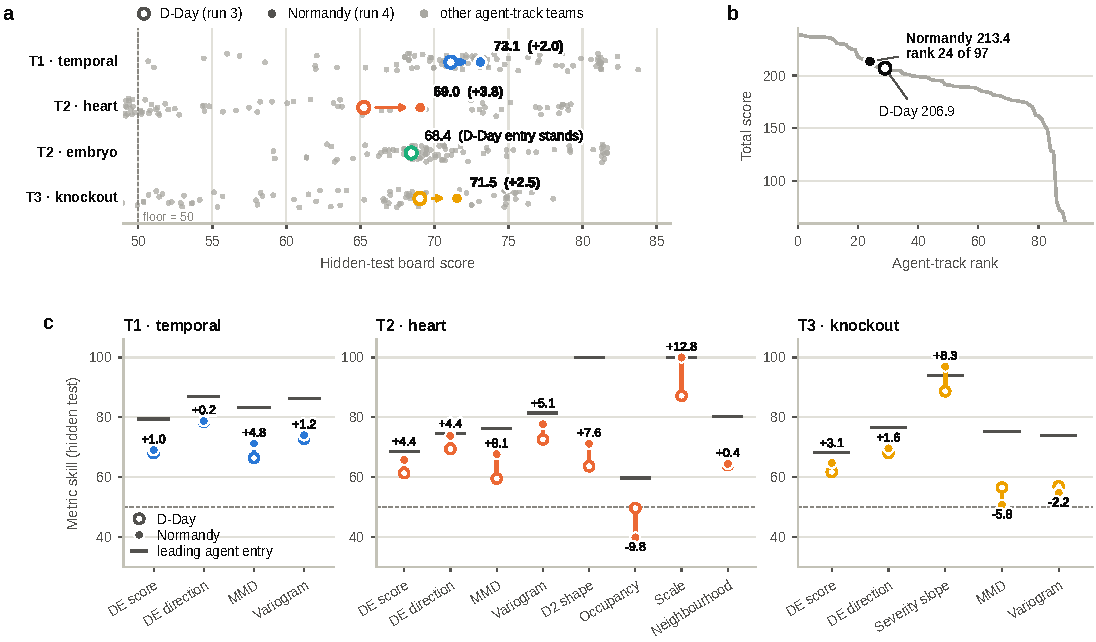
\includegraphics[width=0.84\textwidth]{fig/fig_test.pdf}
\caption{\textbf{Hidden-test results} (public leaderboard after submissions closed). \textbf{a},~Board scores of our
two submitted runs against the other Agent-track teams (one grey point per team). \textbf{b},~Total score by
Agent-track rank. \textbf{c},~Metric skills of the two runs on the three boards that changed; horizontal bars give the
leading agent entry on each board, the dashed line the floor. Numbers are the change from run~3 to run~4.}
\label{fig:test}
\end{figure*}

% =====================================================================================================================
\section{Discussion}

\paragraph{Agents optimise the measurement} The agents did what the brief asked: find the metric with the largest gap, form a mechanistic hypothesis and move it. But the development splits differ from the test in horizon and protocol, and a persistent optimiser discovers exactly those differences. Depth thinning that mimics a platform change between two stages, a lineage trend that is a sampling difference between two dissections and a blood content fitted to the one available target were all accepted with tight confidence intervals and plausible biological arguments, and all lost on stages the agents could not see. Paired racing removes noise; it cannot remove bias in what is measured. For autonomous research on small scientific benchmarks we now consider a holdout that agents can neither read nor query the most important component.

\paragraph{A run that returns its seed is a result} Run~3 spent 14 hours and 68 cycles to export the files it had started from. We count this as the selection rule doing its work, since promoting the best of its 21 accepted changes would have cost points on stages that resemble the test. The price is conservatism: with three seed pairs the rule also declined a T1 change whose mean holdout gain was two points.

\paragraph{The lock moves human influence; it does not remove it} The largest single-board test gains between runs~3 and~4 followed changes that people made to the seed after reading the test feedback: the T1 composition fix, the heart organ definition and radius cap, and the T3 deep delay. ``Agent-found'' and ``agent-run'' are different claims. In our entry the agents ran everything after the lock and found the selected T1 and heart changes; the embryo and T3 files are the output of human-prepared seed code.

\paragraph{Limitations} (i)~The T1 holdout was not fully blind: its target stage is contained in the external atlas that agents, though not programs, could read as a prior. (ii)~Each holdout comparison rests on three seed pairs and one target per board, so the bound in Eq.~\ref{eq:lb} covers sampling noise, not target-to-target variation. (iii)~No local split reproduces the test's occupancy behaviour on the embryo board. (iv)~T3 was excluded from research in the final run, and its delay constant was taken from public entry names. (v)~Provider quotas bounded the runs: three quarters of the agent calls of runs~3 and~4 ran on a substitute model. (vi)~The predecessor runs changed their holdouts from run to run and are not pooled with the four runs of Fig.~\ref{fig:transfer}.

% =====================================================================================================================
\section{Agent-track statement and disclosures}

\paragraph{Framework} AgenticScientist, our own multi-role orchestrator, driving vendor command-line agents (Claude
Code, Codex~CLI, Antigravity~CLI, OpenCode and CommandCode) inside a Landlock sandbox.

\paragraph{Models actually run} Run~3 (first submission): \code{gpt-6.2-sol}, \code{claude-opus-5-5},
\code{gemini-4-neon-high}, \code{gpt-6-luna} and \code{deepseek-v4.1-flash} as researchers and reviewers, with
\code{claude-sonnet-5-5} in supporting roles. Its files contain no change made in run~3; the agent changes they
carry were selected in run~1 (T1 and T3 by \code{gpt-6.2-sol}, heart by \code{claude-opus-5-5}) and run~2 (heart,
\code{gpt-6.2-sol}). Run~4 (second submission): the same models and \code{claude-fable-5-2}. The submitted T1
change was written by \code{claude-opus-5-5} and the heart change by \code{claude-fable-5-2}; the embryo and T3
files come from the locked seed.

\paragraph{Human involvement} Before each lock, people wrote the seed program, prompts, evaluation splits, gates and
configuration, using completed earlier runs (including those of Section~\ref{sec:pre}), the test feedback of run~3
and the public leaderboard. After a lock, people changed no input of the run. Runs~2 and~3 were ended by an operator
before their scheduled stop; run~4 ran to schedule. Selection, export and packaging were automatic in every run.
People chose which completed runs to submit and uploaded the files unchanged.

\paragraph{External data} All sources are listed in Table~\ref{tab:data} with their stage filters. Agents could also read an extended gastrulation atlas \cite{imaz2024extended} and pretrained gene embeddings \cite{theodoris2023geneformer}; neither is read by the submitted programs. Public leaderboard entry names and scores were used as evidence by people and agents. No measured data from the held-out test stages were used by any route.

\paragraph{Evidence} Each submission carries the complete trajectory of agent calls, all prompts, the harness source
and a manifest binding the lock, the selected workspace and the SHA-256 of every exported file.

\section*{Acknowledgements}
\noindent We thank the organisers of the Virtual Embryo Challenge for the benchmark, the scoring code and the public
leaderboard, and Dr.~Qingquan Zhang and Dr.~Neil Chi and their team for generating the challenge data. We thank the
authors of the public atlases used as priors.

% =====================================================================================================================
{\sffamily\fontsize{7.1}{8.7}\selectfont
\begin{thebibliography}{99}
\setlength{\itemsep}{1.5pt}

\bibitem{lu2024aiscientist} Lu, C. \emph{et al.} The AI Scientist: towards fully automated open-ended scientific
discovery. Preprint at \url{https://arxiv.org/abs/2408.06292} (2024).

\bibitem{romera2024funsearch} Romera-Paredes, B. \emph{et al.} Mathematical discoveries from program search with large
language models. \emph{Nature} \textbf{625}, 468--475 (2024).

\bibitem{novikov2025alphaevolve} Novikov, A. \emph{et al.} AlphaEvolve: a coding agent for scientific and algorithmic
discovery. Preprint at \url{https://arxiv.org/abs/2506.13131} (2025).

\bibitem{dwork2015reusable} Dwork, C. \emph{et al.} The reusable holdout: preserving validity in adaptive data
analysis. \emph{Science} \textbf{349}, 636--638 (2015).

\bibitem{blum2015ladder} Blum, A. \& Hardt, M. The Ladder: a reliable leaderboard for machine learning competitions.
In \emph{Proc.\ 32nd Int.\ Conf.\ Machine Learning} 1006--1014 (PMLR, 2015).

\bibitem{vec2026} Virtual Embryo Challenge. Overview, rules and evaluation. \url{https://virtualembryo.ai/challenge}
(accessed 26 November 2026).

\bibitem{gretton2012kernel} Gretton, A., Borgwardt, K. M., Rasch, M. J., Sch\"olkopf, B. \& Smola, A. A kernel
two-sample test. \emph{J.\ Mach.\ Learn.\ Res.} \textbf{13}, 723--773 (2012).

\bibitem{lange2025shinka} Lange, R. T., Imajuku, Y. \& Cetin, E. ShinkaEvolve: towards open-ended and sample-efficient
program evolution. Preprint at \url{https://arxiv.org/abs/2509.19349} (2025).

\bibitem{salaun2017landlock} Sala\"un, M. Landlock: unprivileged access control. Linux kernel documentation,
\url{https://docs.kernel.org/userspace-api/landlock.html}.

\bibitem{snoek2012practical} Snoek, J., Larochelle, H. \& Adams, R. P. Practical Bayesian optimization of machine
learning algorithms. In \emph{Advances in Neural Information Processing Systems} \textbf{25}, 2951--2959 (2012).

\bibitem{birattari2002racing} Birattari, M., St\"utzle, T., Paquete, L. \& Varrentrapp, K. A racing algorithm for
configuring metaheuristics. In \emph{Proc.\ Genetic and Evolutionary Computation Conf.} 11--18 (2002).

\bibitem{qiu2024timelapse} Qiu, C. \emph{et al.} A single-cell time-lapse of mouse prenatal development from gastrula
to birth. \emph{Nature} \textbf{626}, 1084--1093 (2024).

\bibitem{feulner2024} Feulner, L. \emph{et al.} Perinatal mouse heart single-cell atlas (GEO GSE150817). Preprint at
\url{https://doi.org/10.1101/2024.03.05.583423} (2024).

\bibitem{ashburner2000go} Ashburner, M. \emph{et al.} Gene Ontology: tool for the unification of biology.
\emph{Nat.\ Genet.} \textbf{25}, 25--29 (2000).

\bibitem{desoysa2019} de Soysa, T. Y. \emph{et al.} Single-cell analysis of cardiogenesis reveals basis for
organ-level developmental defects. \emph{Nature} \textbf{572}, 120--124 (2019).

\bibitem{muncievasic2025} Muncie-Vasic, J. M. \emph{et al.} \emph{Mef2c}-null heart tube single-nucleus data set (GEO
GSE280543). \emph{Genes Dev.} (2025).

\bibitem{imaz2024extended} Imaz-Rosshandler, I. \emph{et al.} Tracking early mammalian organogenesis: prediction and
validation of differentiation trajectories at whole organism scale. \emph{Development} \textbf{151}, dev201867 (2024).

\bibitem{theodoris2023geneformer} Theodoris, C. V. \emph{et al.} Transfer learning enables predictions in network
biology. \emph{Nature} \textbf{618}, 616--624 (2023).

\end{thebibliography}}

\end{document}
